\section{REAPER - Melanie B. Sigl}


\begin{frame}
	\frametitle{REAPER - Deep Transfer Learning Model Selection in a Time Series Modeling Context}

	\begin{columns}
		\begin{column}{0.4\textwidth}
			\begin{flushleft}
				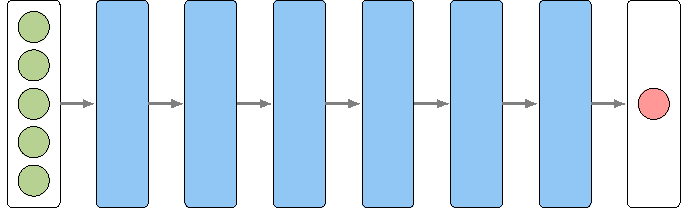
\includegraphics[height=5.5em,page=1]{img/research/reaper-tl-base.pdf}
			\end{flushleft}
			\vspace*{0.5em}
			\begin{flushleft}
				\includegraphics[height=5.5em,page=2]{img/research/reaper-tl-base.pdf}
			\end{flushleft}

			\begin{tikzpicture}[overlay]
				\node[draw,rectangle,minimum width=16.25em, minimum height=6em, rounded corners=.25em] at (2.55,4.2) (base) {};
				\node[draw,rectangle,minimum width=16.25em, minimum height=6em, rounded corners=.25em] at (2.55,1.62) (transfer) {};
				\draw[->,thick] (base) edge (transfer);
				\node[fill=white, below right=0.1em and -8em of base] {\small transfer};
			\end{tikzpicture}
		\end{column}

		\begin{column}{0.6\textwidth}
			\vspace*{-4.5em}
			\begin{flushleft}
				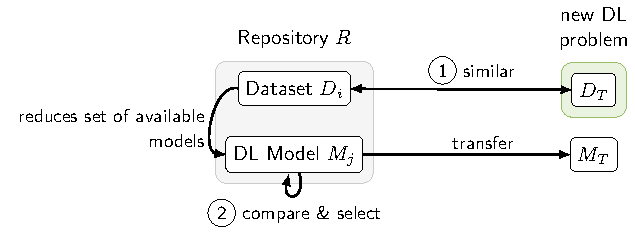
\includegraphics[width=\textwidth]{img/research/reaper-method.pdf}
			\end{flushleft}

			\begin{center}
				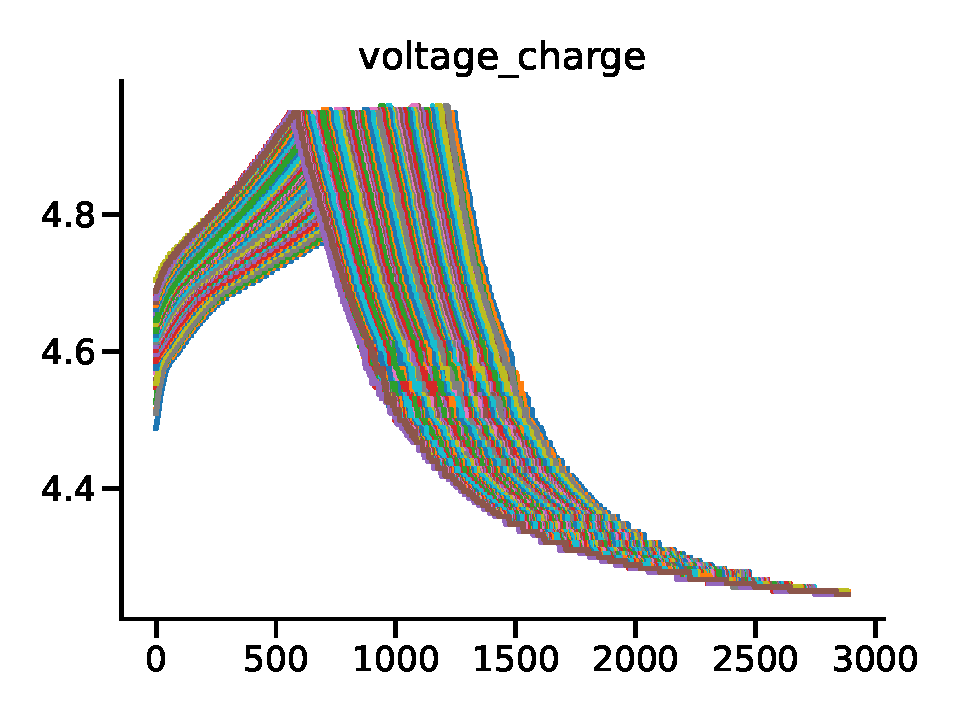
\includegraphics[width=0.4\textwidth]{img/research/reaper-voltage-charge_cycles.pdf}
				\hspace*{1em}
				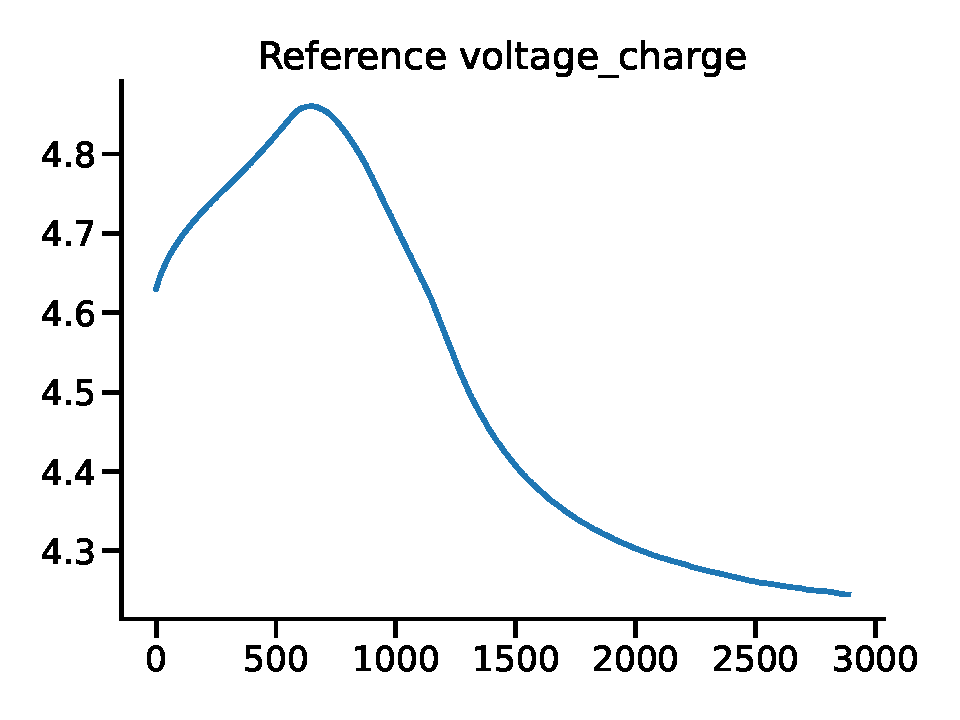
\includegraphics[width=0.4\textwidth]{img/research/reaper-voltage-charge-dba.pdf}
			\end{center}
		\end{column}
	\end{columns}

\end{frame}
